\documentclass[10pt,oneside]{article}
\usepackage[T1]{fontenc}
\usepackage[utf8]{inputenc}
% \usepackage{lmodern}
%\usepackage[adobe-utopia,uppercase=upright,greeklowercase=upright]{mathdesign}
\usepackage[adobe-utopia]{mathdesign}
%\usepackage{minionpro}
% \usepackage{pifont}
% \usepackage{amssymb}
\usepackage{amsmath}
\usepackage[francais]{babel}
% \usepackage[francais]{varioref}
\usepackage[dvips]{graphicx}

\usepackage{framed}
\usepackage[normalem]{ulem}
\usepackage{fancyhdr}
\usepackage{titlesec}
\usepackage{vmargin}
\usepackage{longtable}

\usepackage{ifthen}


%\usepackage{epsfig}
\usepackage{subfig}

\usepackage{multirow}
\usepackage{multicol} % Portions de texte en colonnes
\usepackage{flafter}%floatants après la référence



\usepackage{color}
\usepackage{colortbl}


\definecolor{gris25}{gray}{0.75}
\definecolor{bleu}{RGB}{18,33,98}
\definecolor{bleuf}{RGB}{42,94,171}
\definecolor{bleuc}{RGB}{231,239,247}
\definecolor{rougef}{RGB}{185,18,27}
\definecolor{rougec}{RGB}{255,230,231}
\definecolor{vertf}{RGB}{103,126,82}
\definecolor{vertc}{RGB}{220,255,191}
\definecolor{violetf}{RGB}{112,48,160}
\definecolor{violetc}{RGB}{230,224,236}

\newenvironment{sci}[1][\hsize]%
{%
    \def\FrameCommand%
    {%
%\rotatebox{90}{\textit{\textsf{Scilab}}\includegraphics[height=.8cm]{png/logo_scilab}} 
\rotatebox{90}{\includegraphics[height=.6cm]{png/logo_scilab}} 
        {\color{violetf}\vrule width 3pt}%
        \hspace{0pt}%must no space.
        \fboxsep=\FrameSep\colorbox{violetc}%
    }%
    \MakeFramed{\hsize #1 \advance\hsize-\width\FrameRestore}%
}%
{\endMakeFramed}%

\newenvironment{pseudo}[1][\hsize]%
{%
    \def\FrameCommand%
    {%
\rotatebox{90}{\textit{\textsf{Pseudo Code}}} 
        {\color{violetf}\vrule width 3pt}%
        \hspace{0pt}%must no space.
        \fboxsep=\FrameSep\colorbox{violetc}%
    }%
    \MakeFramed{\hsize #1 \advance\hsize-\width\FrameRestore}%
}%
{\endMakeFramed}%

\newenvironment{py}[1][\hsize]%
{%
    \def\FrameCommand%
    {%
%\rotatebox{90}{\textit{\textsf{Python}}} 
\rotatebox{90}{\includegraphics[height=.6cm]{png/logo_python}} 
        {\color{violetf}\vrule width 3pt}%
        \hspace{0pt}%must no space.
        \fboxsep=\FrameSep\colorbox{violetc}%
    }%
    \MakeFramed{\hsize #1 \advance\hsize-\width\FrameRestore}%
}%
{\endMakeFramed}%


\newenvironment{corrige}[1][\hsize]%
{%
    \def\FrameCommand
    {%
\rotatebox{90}{\textit{\textsf{Correction}}} 
        {\color{violetf}\vrule width 3pt}%
        \hspace{0pt}%must no space.
        \fboxsep=\FrameSep\colorbox{violetc}%
    }%
    \MakeFramed{\hsize#1\advance\hsize-\width\FrameRestore}%
}%
{\endMakeFramed}%



\newenvironment{rem}[1][\hsize]%
{%
    \def\FrameCommand
    {%
\rotatebox{90}{\textit{\textsf{Remarque}}} 
        {\color{bleuf}\vrule width 3pt}%
        \hspace{0pt}%must no space.
        \fboxsep=\FrameSep\colorbox{bleuc}%
    }%
    \MakeFramed{\hsize#1\advance\hsize-\width\FrameRestore}%
}%
{\endMakeFramed}%


\newenvironment{savoir}[1][\hsize]%
{%
    \def\FrameCommand
    {%
\rotatebox{90}{\textit{\textsf{Savoir}}} 
        {\color{bleuf}\vrule width 3pt}%
        \hspace{0pt}%must no space.
        \fboxsep=\FrameSep\colorbox{bleuc}%
    }%
    \MakeFramed{\hsize#1\advance\hsize-\width\FrameRestore}%
}%
{\endMakeFramed}%

\newenvironment{prob}[1][\hsize]%
{%
    \def\FrameCommand%
    {%
\rotatebox{90}{\textit{\textsf{ Problématique}}} 
        {\color{rougef}\vrule width 3pt}%
        \hspace{0pt}%must no space.
        \fboxsep=\FrameSep\colorbox{rougec}%
    }%
    \MakeFramed{\hsize#1\advance\hsize-\width\FrameRestore}%
}%
{\endMakeFramed}%

\newenvironment{obj}[1][\hsize]%
{%
    \def\FrameCommand%
    {%
\rotatebox{90}{\textit{\textsf{ $\;$}}} 
        {\color{rougef}\vrule width 3pt}%
        \hspace{0pt}%must no space.
        \fboxsep=\FrameSep\colorbox{rougec}%
    }%
    \MakeFramed{\hsize#1\advance\hsize-\width\FrameRestore}%
}%
{\endMakeFramed}%

\newenvironment{defi}[1][\hsize]%
{%
    \def\FrameCommand%
    {%
\rotatebox{90}{\textit{\textsf{Définition\\}}} 
        {\color{bleuf}\vrule width 3pt}%
        \hspace{0pt}%must no space.
        \fboxsep=\FrameSep\colorbox{bleuc}%
    }%
    \MakeFramed{\hsize#1\advance\hsize-\width\FrameRestore}%
}%
{\endMakeFramed}%


\newenvironment{demo}[1][\hsize]%
{%
    \def\FrameCommand%
    {%
\rotatebox{90}{\textit{\textsf{Démonstration\\}}} 
        {\color{bleuf}\vrule width 3pt}%
        \hspace{0pt}%must no space.
        \fboxsep=\FrameSep\colorbox{bleuc}%
    }%
    \MakeFramed{\hsize#1\advance\hsize-\width\FrameRestore}%
}%
{\endMakeFramed}%


\newenvironment{hypo}[1][\hsize]%
{%
    \def\FrameCommand%
    {%
\rotatebox{90}{\textit{\textsf{Hypothèse\\}}} 
        {\color{bleuf}\vrule width 3pt}%
        \hspace{0pt}%must no space.
        \fboxsep=\FrameSep\colorbox{bleuc}%
    }%
    \MakeFramed{\hsize#1\advance\hsize-\width\FrameRestore}%
}%
{\endMakeFramed}%


\newenvironment{prop}[1][\hsize]%
{%
    \def\FrameCommand%
    {%
\rotatebox{90}{\textit{\textsf{Propriété\\}}} 
        {\color{bleuf}\vrule width 3pt}%
        \hspace{0pt}%must no space.
        \fboxsep=\FrameSep\colorbox{bleuc}%
    }%
    \MakeFramed{\hsize#1\advance\hsize-\width\FrameRestore}%
}%
{\endMakeFramed}%

\newenvironment{props}[1][\hsize]%
{%
    \def\FrameCommand%
    {%
\rotatebox{90}{\textit{\textsf{Propriétés\\}}} 
        {\color{bleuf}\vrule width 3pt}%
        \hspace{0pt}%must no space.
        \fboxsep=\FrameSep\colorbox{bleuc}%
    }%
    \MakeFramed{\hsize#1\advance\hsize-\width\FrameRestore}%
}%
{\endMakeFramed}%

\newenvironment{exemple}[1][\hsize]%
{%
    \def\FrameCommand%
    {%
\rotatebox{90}{\textit{\textsf{Exemple\\}}} 
        {\color{vertf}\vrule width 3pt}%
        \hspace{0pt}%must no space.
        \fboxsep=\FrameSep\colorbox{vertc}%
    }%
    \MakeFramed{\hsize#1\advance\hsize-\width\FrameRestore}%
}%
{\endMakeFramed}%

\newenvironment{resultat}[1][\hsize]%
{%
    \def\FrameCommand%
    {%
\rotatebox{90}{\textit{\textsf{Résultat\\}}} 
        {\color{rougef}\vrule width 3pt}%
        \hspace{0pt}%must no space.
        \fboxsep=\FrameSep\colorbox{rougec}%
    }%
    \MakeFramed{\hsize#1\advance\hsize-\width\FrameRestore}%
}%
{\endMakeFramed}%

\newenvironment{methode}[1][\hsize]%
{%
    \def\FrameCommand%
    {%
\rotatebox{90}{\textit{\textsf{Méthode\\}}} 
        {\color{rougef}\vrule width 3pt}%
        \hspace{0pt}%must no space.
        \fboxsep=\FrameSep\colorbox{rougec}%
    }%
    \MakeFramed{\hsize#1\advance\hsize-\width\FrameRestore}%
}%
{\endMakeFramed}%

\newenvironment{theo}[1][\hsize]%
{%
    \def\FrameCommand%
    {%
\rotatebox{90}{\textit{\textsf{Théorème\\}}} 
        {\color{rougef}\vrule width 3pt}%
        \hspace{0pt}%must no space.
        \fboxsep=\FrameSep\colorbox{rougec}%
    }%
    \MakeFramed{\hsize#1\advance\hsize-\width\FrameRestore}%
}%
{\endMakeFramed}%

\newenvironment{warn}[1][\hsize]%
{%
    \def\FrameCommand%
    {%
\rotatebox{90}{\textit{\textsf{Attention\\}}} 
        {\color{rougef}\vrule width 3pt}%
        \hspace{0pt}%must no space.
        \fboxsep=\FrameSep\colorbox{rougec}%
    }%
    \MakeFramed{\hsize#1\advance\hsize-\width\FrameRestore}%
}%
{\endMakeFramed}%

% \usepackage{pstricks}
%\usepackage{minitoc}
% \setcounter{minitocdepth}{4}

\setcounter{tocdepth}{2}

% \mtcselectlanguage{french} 

%\usepackage{draftcopy}% "Brouillon"
% \usepackage{floatflt}
\usepackage{psfrag}
%\usepackage{listings} % Permet d'insérer du code de programmation
\renewcommand{\baselinestretch}{1.2}

% Changer la numérotation des figures :
% ------------------------------------
% \makeatletter
% \renewcommand{\thefigure}{\ifnum \c@section>\z@ \thesection.\fi
%  \@arabic\c@figure}
% \@addtoreset{figure}{section}
% \makeatother
 


%%%%%%%%%%%%
% Définition des vecteurs %
%%%%%%%%%%%%
 \newcommand{\vect}[1]{\overrightarrow{#1}}

%%%%%%%%%%%%
% Définition des torseusr %
%%%%%%%%%%%%

 \newcommand{\torseur}[1]{%
\left\{{#1}\right\}
}

\newcommand{\torseurcin}[3]{%
\left\{\mathcal{#1} \left(#2/#3 \right) \right\}
}

\newcommand{\torseurstat}[3]{%
\left\{\mathcal{#1} \left(#2\rightarrow #3 \right) \right\}
}

 \newcommand{\torseurc}[8]{%
%\left\{#1 \right\}=
\left\{
{#1}
\right\}
 = 
\left\{%
\begin{array}{cc}%
{#2} & {#5}\\%
{#3} & {#6}\\%
{#4} & {#7}\\%
\end{array}%
\right\}_{#8}%
}

 \newcommand{\torseurcol}[7]{
\left\{%
\begin{array}{cc}%
{#1} & {#4}\\%
{#2} & {#5}\\%
{#3} & {#6}\\%
\end{array}%
\right\}_{#7}%
}

 \newcommand{\torseurl}[3]{%
%\left\{\mathcal{#1}\right\}_{#2}=%
\left\{%
\begin{array}{l}%
{#1} \\%
{#2} %
\end{array}%
\right\}_{#3}%
}

 \newcommand{\vectv}[3]{%
\vect{V\left( {#1} \in {#2}/{#3}\right)}
}


\newcommand{\vectf}[2]{%
\vect{R\left( {#1} \rightarrow {#2}\right)}
}

\newcommand{\vectm}[3]{%
\vect{\mathcal{M}\left( {#1}, {#2} \rightarrow {#3}\right)}
}


 \newcommand{\vectg}[3]{%
\vect{\Gamma \left( {#1} \in {#2}/{#3}\right)}
}

 \newcommand{\vecto}[2]{%
\vect{\Omega\left( {#1}/{#2}\right)}
}
% }$$\left\{\mathcal{#1} \right\}_{#2} =%
% \left\{%
% \begin{array}{c}%
%  #3 \\%
%  #4 %
% \end{array}%
% \right\}_{#5}}

%  ------------------------------------------
% | Modification du formatage des sections : | 
%  ------------------------------------------

% Grands titres :
% ---------------

\newcommand{\titre}[1]{%
\begin{center}
      \bigskip
      \rule{\textwidth}{1pt}
      \par\vspace{0.1cm}
      
      \textbf{\large #1}
      \par\rule{\textwidth}{1pt}
    \end{center}
    \bigskip
  }

% Supprime le numéro du chapitre dans la numérotation des sections:
% -----------------------------------------------------------------
\makeatletter
\renewcommand{\thesection}{\@arabic\c@section}
\makeatother


% \titleformat{\chapter}[display]
% {\normalfont\Large\filcenter}
% {}
% {1pc}
% {\titlerule[1pt]
%   \vspace{1pc}%
%   \Huge}[\vspace{1ex}%
% \titlerule]


%%%% Chapitres Comme PY Pechard %%%%%%%%%
% numéro du chapitre
\DeclareFixedFont{\chapnumfont}{OT1}{phv}{b}{n}{80pt}
% pour le mot « Chapitre »
\DeclareFixedFont{\chapchapfont}{OT1}{phv}{m}{it}{40pt}
% pour le titre
\DeclareFixedFont{\chaptitfont}{T1}{phv}{b}{n}{25pt}

\definecolor{gris}{gray}{0.75}
\titleformat{\chapter}[display]%
	{\sffamily}%
	{\filleft\chapchapfont\color{gris}\chaptertitlename\
	\\
	\vspace{12pt}
	\chapnumfont\thechapter}%
	{16pt}%
	{\filleft\chaptitfont}%
	[\vspace{6pt}\titlerule\titlerule\titlerule]

%%%%  Fin Chapitres Comme PY Pechard %%%%%%%%%


% Section, subsection, subsubsection sans serifs :
% % ----------------------------------------------

% \makeatletter
% \renewcommand{\section}{\@startsection{section}{0}{0mm}%
% {\baselineskip}{.3\baselineskip}%
% {\normalfont\sffamily\Large\textbf}}%
% \makeatother

\makeatletter
\renewcommand{\@seccntformat}[1]{{\textcolor{bleu}{\csname
the#1\endcsname}\hspace{0.5em}}}
\makeatother

\makeatletter
\renewcommand{\section}{\@startsection{section}{1}{\z@}%
                       {-4ex \@plus -1ex \@minus -.4ex}%
                       {1ex \@plus.2ex }%
                       {\normalfont\Large\sffamily\bfseries}}%
\makeatother
 
\makeatletter
\renewcommand{\subsection}{\@startsection {subsection}{2}{\z@}
                          {-3ex \@plus -0.1ex \@minus -.4ex}%
                          {0.5ex \@plus.2ex }%
                          {\normalfont\large\sffamily\bfseries}}
\makeatother
 
\makeatletter
\renewcommand{\subsubsection}{\@startsection {subsubsection}{3}{\z@}
                          {-2ex \@plus -0.1ex \@minus -.2ex}%
                          {0.2ex \@plus.2ex }%
                          {\normalfont\large\sffamily\bfseries}}
\makeatother
 
\makeatletter             
\renewcommand{\paragraph}{\@startsection{paragraph}{4}{\z@}%
                                    {-2ex \@plus-.2ex \@minus .2ex}%
                                    {0.1ex}%               
{\normalfont\sffamily\bfseries}}
\makeatother
 

\makeatletter             
\renewcommand{\subparagraph}{\@startsection{subparagraph}{5}{\z@}%
                                    {-2ex \@plus-.2ex \@minus .2ex}%
                                    {0.1ex}%               
{\normalfont\bfseries Question }}
\makeatother

\renewcommand{\thesubparagraph}{\arabic{subparagraph}} 
%
\makeatletter
%\renewcommand{\subparagraph}{\@startsection{subparagraph}{5}{\z@}%
%                                       {-2ex \@plus-.1ex \@minus .2ex}%
%                                       {0.1ex}%
%				    {\normalfont\normalsize\sffamily\bfseries}}
%\makeatletter
% \makeatletter
% \renewcommand{\subsection}{\@startsection{subsection}{1}{2mm}%
% {\baselineskip}{.3\baselineskip}%
% {\normalfont\sffamily\large\textbf}}%
% \makeatother
% 
% \makeatletter
% \renewcommand{\subsubsection}{\@startsection{subsubsection}{2}{4mm}%
% {\baselineskip}{.15\baselineskip}%
% {\normalfont\sffamily\large\textbf}}%
% \makeatother
% 
% \makeatletter
% \renewcommand{\paragraph}{\@startsection{paragraph}{3}{6mm}%
% {\baselineskip}{.15\baselineskip}%
% {\normalfont\sffamily\large\textbf}}%
% \makeatother
 
\setcounter{secnumdepth}{5}


%  --------
% | Marges |
%  --------


% \setmarginsrb{2.5cm}{1.5cm}{2.5cm}{2cm}{1cm}{1cm}{1cm}{1cm}
\setmarginsrb{1.5cm}{1cm}{1cm}{1.5cm}{1cm}{1cm}{1cm}{1cm}

% Changer les marges localement :
% -----------------------------
\newenvironment{changemargin}[2]{\begin{list}{}{%
\setlength{\topsep}{0pt}%
\setlength{\leftmargin}{0pt}%
\setlength{\rightmargin}{0pt}%
\setlength{\listparindent}{\parindent}%
\setlength{\itemindent}{\parindent}%
\setlength{\parsep}{0pt plus 1pt}%
\addtolength{\leftmargin}{#1}%
\addtolength{\rightmargin}{#2}%
}\item }{\end{list}}



\usepackage{pst-solides3d}
\usepackage{titletoc}
\titlecontents{chapter}[+3pc]
  {\addvspace{10pt}\sffamily\bfseries}
{\contentslabel[{\pscirclebox[fillstyle=solid,fillcolor=gray!25,
linecolor=gray!25,framesep=4pt]{\textcolor{white}{\thecontentslabel}}}]{2.5pc}}
  {}
  {\dotfill \normalfont\thecontentspage\ }

\titlecontents{section}[3pc]
  {\addvspace{2pt}\sffamily}
  {\contentslabel[\thecontentslabel]{1.8pc}}
  {}
  {\dotfill \normalfont\thecontentspage\ }

\titlecontents{subsection}[5pc]
  {\addvspace{2pt}\sffamily}
  {\contentslabel[\thecontentslabel]{1.8pc}}
  {}
  {\dotfill \normalfont\thecontentspage\ }

\titlecontents{subsubsection}[8pc]
  {\addvspace{2pt}\sffamily}
  {\contentslabel[\thecontentslabel]{3pc}}
  {}
  {\dotfill \normalfont\thecontentspage\ }
%{\;\titlerule\;\normalfont\thecontentspage\ }

\titlecontents{paragraph}[9pc]
  {\addvspace{2pt}\sffamily}
  {\contentslabel[\thecontentslabel]{3.5pc}}
  {}
  {\dotfill \normalfont\thecontentspage\ }





%Si le boolen xp est vrai : compilation pour xabi
%Sinon compilation Damien
\newboolean{xp}
\setboolean{xp}{true}

\newboolean{prof}
\setboolean{prof}{true}

\def\xxtitre{\ifthenelse{\boolean{xp}}{
CI 3 -- CIN : Étude du comportement cinématique des systèmes}{
}}

\def\xxsoustitre{\ifthenelse{\boolean{xp}}{
Chapitre 4 -- Étude des chaînes fermées :

Détermination des lois Entrée -- Sortie}{
}}


\def\xxauteur{\ifthenelse{\boolean{xp}}{
\noindent 2013 -- 2014 \\
Xavier \textsc{Pessoles}}{
}}


\def\xxpied{\ifthenelse{\boolean{xp}}{
CI 4 : CIN -- Cours \\
Ch 4 : Chaînes fermées -- Loi entrée -- sortie -- \ifthenelse{\boolean{prof}}{P}{E}%
}{
}}

\usepackage[%
    pdftitle={CIN : Chaînes fermées -- Loi entrée -- sortie},
    pdfauthor={Xavier Pessoles},
    colorlinks=true,
    linkcolor=blue,
    citecolor=magenta]{hyperref}


\usepackage{pifont}
\sloppy
\hyphenpenalty 10000


\begin{document}






% \makeatletter \let\ps@plain\ps@empty \makeatother
%% DEBUT DU DOCUMENT
%% =================




%------------- En tetes et Pieds de Pages ------------


\pagestyle{fancy}
\ifthenelse{\boolean{xp}}{%
\renewcommand{\headrulewidth}{0pt}}{%
\renewcommand{\headrulewidth}{0.2pt}} %pour mettre le trait en haut
%\renewcommand{\headrulewidth}{0.2pt}

\fancyhead{}
\fancyhead[L]{%
\ifthenelse{\boolean{xp}}{%
\noindent\begin{minipage}[c]{2.6cm}%

\includegraphics[width=2cm]{png/logo_ptsi.png}%
\end{minipage}%
}{%
\footnotesize{\textit{\textsf{Lycée François Premier}}}
}}

\ifthenelse{\boolean{xp}}{%
\fancyhead[C]{\rule{12cm}{.5pt}}}{
}


\fancyhead[R]{%
\noindent\begin{minipage}[c]{3cm}
\begin{flushright}
\footnotesize{\textit{\textsf{Sciences Industrielles \\ de l'ingénieur}}}%
\end{flushright}
\end{minipage}
}


\ifthenelse{\boolean{xp}}{%
\fancyhead[C]{\rule{12cm}{.5pt}}}{
}

\renewcommand{\footrulewidth}{0.2pt}

\fancyfoot[C]{\footnotesize{\bfseries \thepage}}
\fancyfoot[L]{%
\begin{minipage}[c]{.2\linewidth}
\noindent\footnotesize{{\xxauteur}}
\end{minipage}
\ifthenelse{\boolean{xp}}{}{%
\begin{minipage}[c]{.15\linewidth}
\includegraphics[width=2cm]{png/logoCC.png}
\end{minipage}}
}


\fancyfoot[R]{\footnotesize{\xxpied}}



\begin{center}
 \huge\textsc{\xxtitre}

\end{center}

\begin{center}
 \LARGE\textsc{\xxsoustitre}
\end{center}


\begin{minipage}[c]{.3\linewidth}
\begin{center}
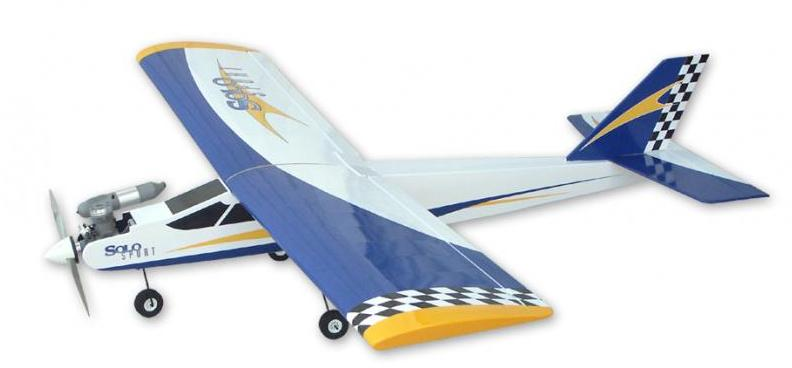
\includegraphics[height=2.5cm]{png/avion}

\textit{Trainer Solo Sport \cite{cite1}} 
\end{center}
\end{minipage} \hfill
\begin{minipage}[c]{.3\linewidth}
\begin{center}
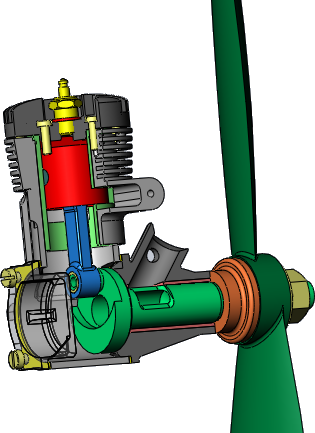
\includegraphics[height=3.5cm]{png/moteur_3d}

\textit{Modèle CAO d'un moteur de modélisme \cite{cite2}}
\end{center}
\end{minipage} \hfill
\begin{minipage}[c]{.3\linewidth}
\begin{center}
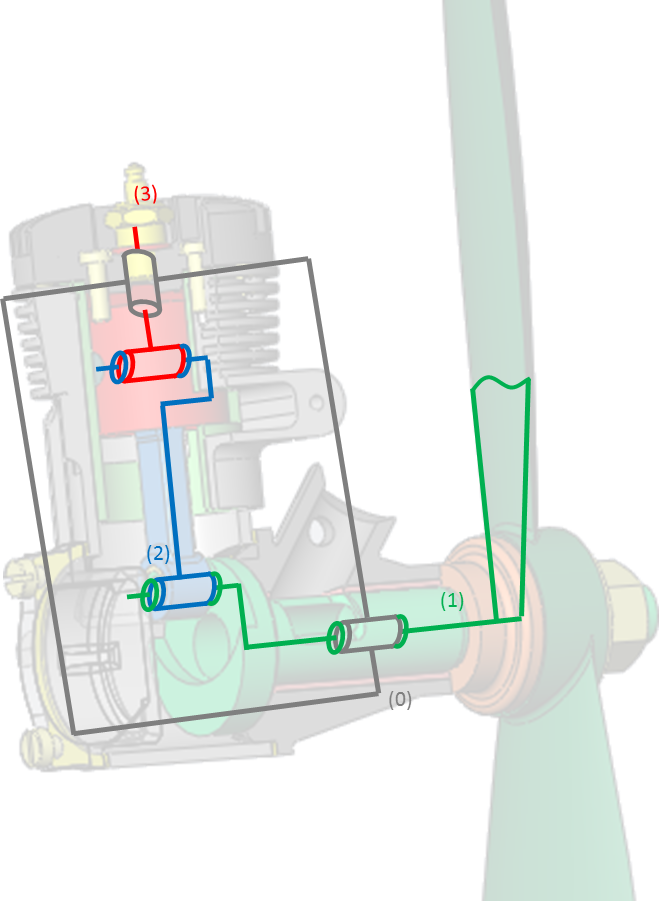
\includegraphics[height=3.5cm]{png/moteur_3d_sch}

\textit{Modélisation par schéma cinématique}
\end{center}
\end{minipage}


\begin{savoir}
\textbf{Savoirs :}
\begin{itemize}
\item Rés-C1.1 : Fermeture géométrique.
\end{itemize}
\end{savoir}

\setlength{\parskip}{0ex plus 0.2ex minus 0ex}
 \renewcommand{\contentsname}{}
 \renewcommand{\baselinestretch}{1}



\textit{Ce document est en évolution permanente. Merci de signaler toutes erreurs ou coquilles.}
\tableofcontents

 \renewcommand{\baselinestretch}{1.2}
\setlength{\parskip}{2ex plus 0.5ex minus 0.2ex}



\section{Chaînes -- Rappel}
\begin{defi}
\textbf{Graphe de structure -- Chaînes}

Graphe qui permet d'avoir une vue d'ensemble du mécanisme :
\begin{itemize}
\item les classes d'équivalences sont schématisées par des cercles avec un repère (celui défini précédemment);
\item les liaisons sont schématisées par des traits qui relient les cercles.
\end{itemize}

On définit 3 types de chaînes :
\begin{center}
\begin{tabular}{ccc}
Les chaînes ouvertes & Les chaînes fermées & Les chaînes complexes \\
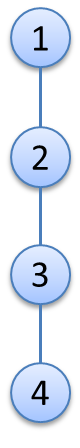
\includegraphics[height=3cm]{png/co.png}
&
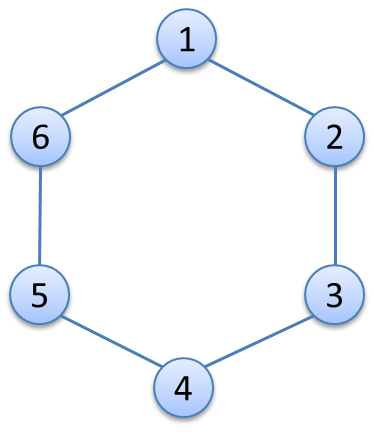
\includegraphics[height=3cm]{png/cf.png}
&
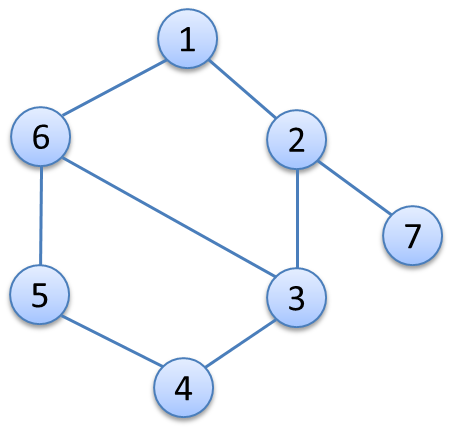
\includegraphics[height=3cm]{png/cc.png}\\
\end{tabular}
\end{center}
\end{defi}

\section{Détermination des lois entrées -- sorties}
\subsection{Introduction}

Dans certains mécanismes, par exemple ceux de transformation de mouvement, les paramètres géométriques peuvent être liés. On choisit donc un paramètre pilote dont on se fixe la valeur ou la loi de variation et par résolution du système d'équations (non linéaire en général donc résolution numérique), on peut trouver le paramètre de sortie.

On s'intéresse donc à l'expression du paramètre de sortie en fonction du paramètre d'entrée. Il n'est donc pas nécessaire, après avoir fixé le paramètre pilote, de calculer tous les autres paramètres variables mais seulement celui de sortie.


\subsection{Fermeture de chaîne angulaire}


\begin{exemple}
\textit{Moteur de modélisme -- Paramétrage}

\begin{center}
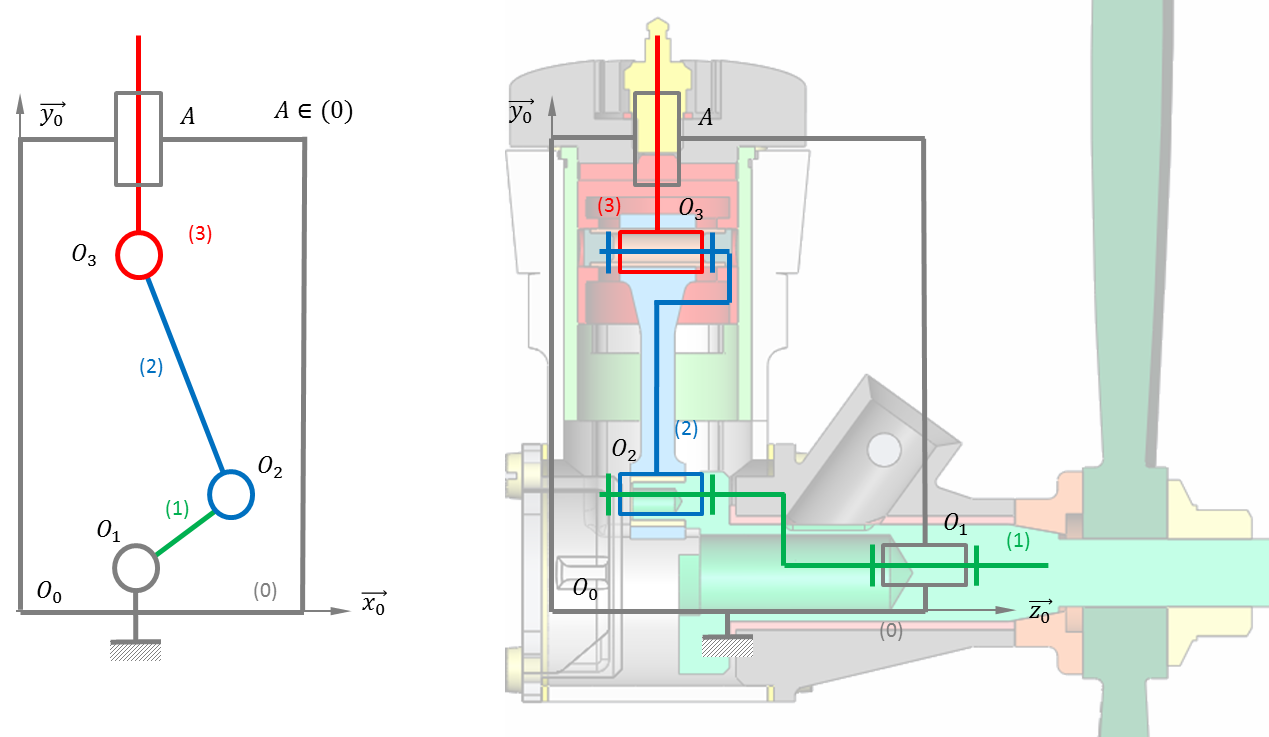
\includegraphics[width=.75\textwidth]{png/moteur_2d_sch}
\end{center}
\begin{center}
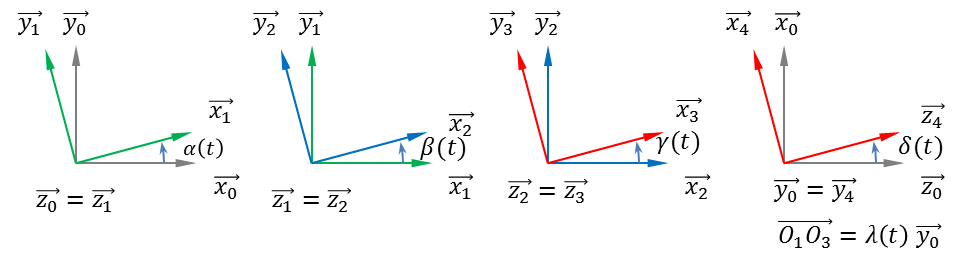
\includegraphics[width=.85\textwidth]{png/param}
\end{center}

Position du point $O_1$ par rapport au point $O_0$ dans le repère $\mathcal{R}_0$ : 
$ \vect{O_0 O_1}= a\vect{x_0}+b\vect{y_0}+c\vect{z_0} $

Position du point $O_2$ par rapport au point $O_1$ dans le repère $\mathcal{R}_1$ : 
$ \vect{O_1 O_2}(t)= d\vect{x_1} $


Position du point $O_3$ par rapport au point $O_2$ dans le repère $\mathcal{R}_2$ : 
$ \vect{O_2 O_3}= e\vect{x_2} $

%Le point $O_2$ est donc immobile dans le repère $\mathcal{R}_1$.

%Position du point $O_2$ par rapport au point $O_1$ dans le repère $\mathcal{R}_0$ : 
%$$
%\vect{O_1 O_2}(t)= d\vect{x_1}=d\cos\alpha(t)\vect{x_0}+d\sin\alpha(t)\vect{y_0}
%$$

%Le point $O_2$ décrit donc un cercle dans le repère $\mathcal{R}_0$.

\end{exemple}


\begin{exemple}
\textit{Moteur de modélisme -- Fermeture angulaire}

\begin{minipage}[c]{.6\linewidth}
Le système a été paramétré ci-dessus. 

On peut définir l'angle $\varphi(t)$ ainsi :
$$
\gamma(t)
=\pi + \left(\dfrac{\pi}{2}-\varphi(t)\right)
= \dfrac{3 \pi}{2}-\varphi(t)
$$
Dans le triangle $O_1 O_2 O_3$, la somme des angles est $\pi$, on a donc : 
$$
\left( \dfrac{\pi}{2} - \alpha(t) \right) + \left(\pi-\beta(t)\right) + \varphi = \pi
\Longleftrightarrow
\left( \dfrac{\pi}{2} - \alpha(t) \right) + \left(\pi-\beta(t)\right) +  \dfrac{3 \pi}{2}-\gamma(t) = \pi
$$

$$
2\pi - \alpha(t) -\beta(t) -\gamma(t) = 0
$$


\end{minipage}\hfill
\begin{minipage}[c]{.35\linewidth}
\begin{center}
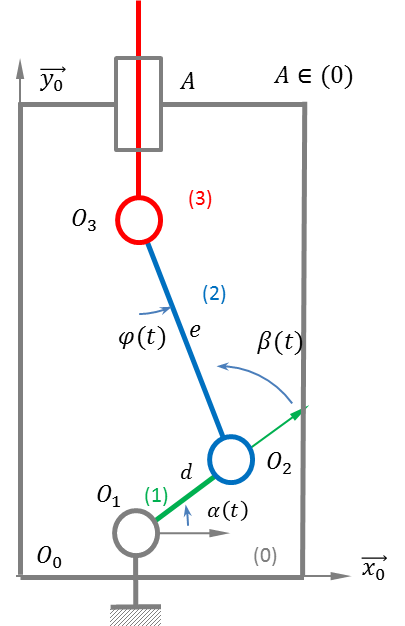
\includegraphics[width=.9\textwidth]{png/chaine}
\end{center}
\end{minipage}
\end{exemple}

\subsection{Fermeture de chaîne géométrique}


\begin{methode}
\textbf{Calcul de la loi Entrée -- Sortie dans une chaîne de solides fermée}

Un système se présentant sous forme d'une chaîne de solide fermée a pour but de transformer un mouvement. On s'intéresse alors pour cela à la relation cinématique liant le mouvement d'entrée du système et le mouvement de sortie. On écrit pour cela une \textbf{fermeture de chaîne géométrique}. Pour cela :
\begin{enumerate}
\item paramétrer le mécanisme;
\item identifier la grandeur d'entrée et de sortie;
\item à l'aide du théorème de Chasles, exprimer le vecteur nul en fonction des vecteurs liant le centre de chacune des liaisons;
\item projeter la relation vectorielle sur une des bases;
\item combiner les relations pour exprimer la sortie en fonction de l'entrée;
\item dériver si besoin pour avoir le lien entre les vitesses. 
\end{enumerate}
\end{methode}


\begin{methode}
\textbf{Méthodes pour manipuler les systèmes équations :} 
\begin{enumerate}
\item Pour supprimer $\lambda$ : on met les deux équations sous la forme $\lambda =$ et on fait le rapport des deux équations.
\item Pour supprimer $\varphi$ : on met une équation sous la forme $\cos\varphi = $ et la seconde sous la forme $\sin\varphi = $ et on utilise la relation $\cos^2\varphi +\sin^2\varphi =1 $.
\item Dans d'autres cas, on peut avoir à utiliser l'expression de la tangente.
\end{enumerate}
\end{methode}


\begin{exemple}


Dans le cas d'un système bielle-manivelle comme le moteur de modélisme, on veut connaître la vitesse de rotation de l'hélice $\dot{\alpha}(t)$ en fonction de la vitesse de translation du piston $\dot{\lambda}(t)$. 

La fermeture géométrique est donc la suivante : 
\begin{eqnarray*}
\vect{O_1 O_2} + \vect{O_2 O_3} +\vect{O_3 O_1} = \vect{0} \\
\Longleftrightarrow d\vect{x_1} + e \vect{x_2} - \lambda(t) \vect{y_0}  = \vect{0}
\end{eqnarray*}

Exprimons $\vect{x_1}$ et $\vect{x_2}$ dans la base $\mathcal{R}_0$ :
$$
\left\{
\begin{array}{lcl}
\vect{x_1} & = & \cos \alpha(t) \vect{x_0} + \sin \alpha(t) \vect{y_0} \\
\vect{x_2} & = & \cos \beta(t) \vect{x_1} + \sin \beta(t) \vect{y_1} \\
 & = & \cos \beta(t) \left( \cos \alpha(t) \vect{x_0} + \sin \alpha(t) \vect{y_0} \right) + 
\sin \beta(t) \left( \cos \alpha(t) \vect{y_0} - \sin \alpha(t) \vect{x_0} \right) \\
\end{array}
\right.
$$
En projetant l'équation vectorielle sur $\vect{x_0}$ et $\vect{y_0}$ on a : 
$$
\left\{
\begin{array}{l}
d\cos\alpha + e \cos\beta \cos\alpha - e \sin\beta \sin\alpha = 0 \\
d\sin\alpha +  e \cos\beta \sin\alpha + e \sin\beta \cos\alpha- \lambda= 0 \\
\end{array}
\right.
\Longleftrightarrow 
\left\{
\begin{array}{l}
d\cos\alpha+ e \cos\left(\beta +\alpha\right)  = 0 \\
d\sin\alpha +  e \sin\left(\beta +\alpha\right) - \lambda= 0 \\
\end{array}
\right.
\Longleftrightarrow 
\left\{
\begin{array}{l}
e \cos\left(\beta +\alpha\right)  = - \dfrac{d\cos\alpha}{e} \\
e \sin\left(\beta +\alpha\right) =  \dfrac{\lambda - d\sin\alpha}{e}
\end{array}
\right.
$$

En passant au carré et en sommant les deux expressions, on a donc : 
$$
\left(\dfrac{d\cos\alpha}{e}\right)^2 + \left(\dfrac{\lambda - d\sin\alpha}{e}\right)^2 = 1 
\Longleftrightarrow
d^2\cos^2\alpha + \lambda^2 + d^2\sin^2\alpha -2d\lambda\sin\alpha = e^2
$$

$$
\Longleftrightarrow
d^2+ \lambda^2 - 2d\lambda\sin\alpha = e^2
$$
Pour exprimer $\lambda$ en fonction de $\alpha$, il faut donc résoudre une équation du second degré. Pour exprimer $\alpha$ en fonction de $\lambda$, la méthode est directe. 

%Résolvons donc 
%$$
%\lambda^2 +2d\lambda\sin\alpha +d^2- e^2=0
%$$
%On calcule le discriminant :
%$$
%\Delta = 4d^2\sin^2\alpha-4\left( d^2- e^2\right)
%$$

%On a donc 
%$$
%\lambda 
%= \dfrac{-2d\sin\alpha \pm \sqrt{\Delta}}{2}
%= -d\sin\alpha \pm \sqrt{d^2\sin^2\alpha-\left( d^2- e^2\right)}
%$$
\end{exemple}



\subsection{Particularité géométrique du mécanisme}


\begin{methode}
\textbf{Calcul de la loi Entrée -- Particularité géométrique}

Lorqsue le mécanisme a une particularité géométrique qui se traduit sous la forme d'une relation vectorielle, on traduit cette dernière à l'aide du paramétrage.

\end{methode}

\begin{exemple}
\textit{Mélangeur}
\begin{center}
\begin{tabular}{cc}
\textit{Mécanisme en situation} & \textit{Modélisation cinématique} \\
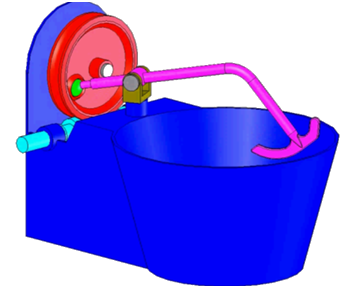
\includegraphics[width=5cm]{png/melangeur_1} & 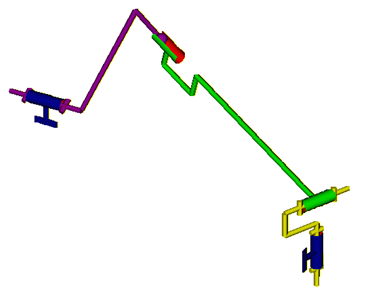
\includegraphics[width=5cm]{png/melangeur_2} \\
& \\
\textit{Réalisation de la liaison linéaure annulaire 1} & \textit{Réalisation de la liaison linéaure annulaire 2} \\ 
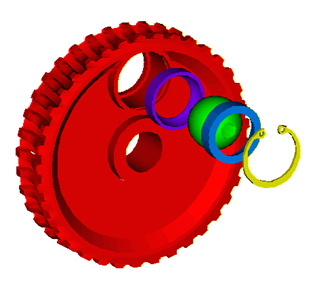
\includegraphics[width=5cm]{png/melangeur_3} & 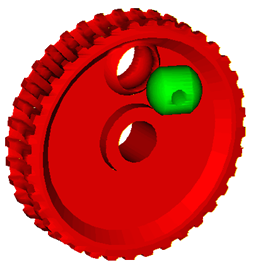
\includegraphics[width=5cm]{png/melangeur_4} \\

\end{tabular}
\end{center}

La pièce 2 tourne entraînant à la sortie un mouvement de rotation oscillant de 4.

\begin{center}
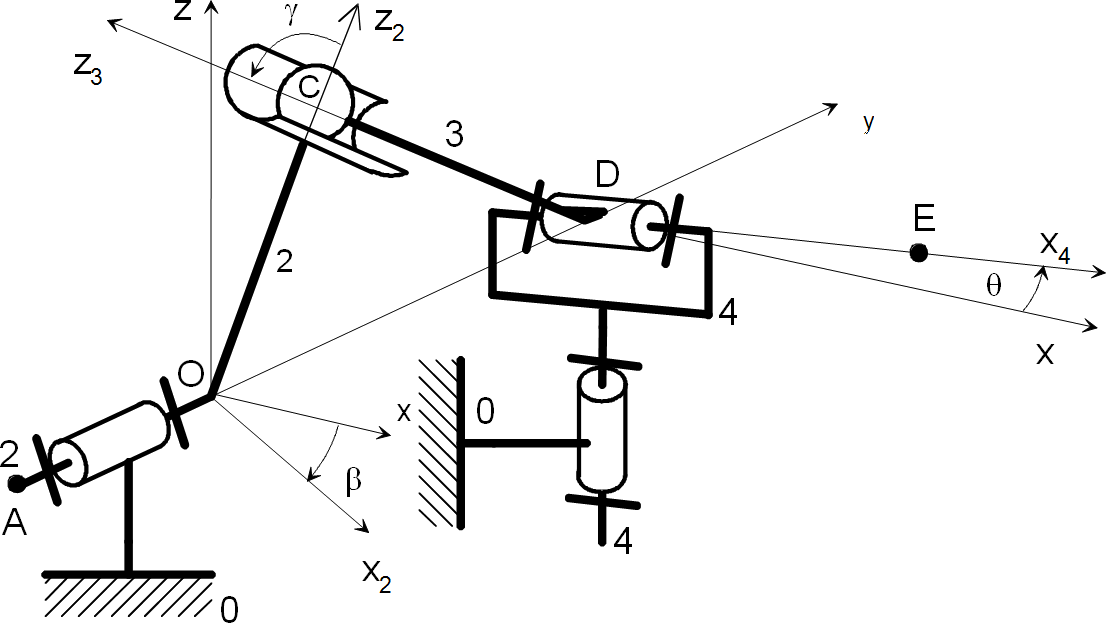
\includegraphics[width=12cm]{png/melangeur_5} 
\end{center}

On donne :
\begin{itemize}
\item soit $\mathcal{R}$ le repère lié au solide 0 considéré comme fixe.$\mathcal{R}=\left(O,\vect{x},\vect{y},\vect{z}\right)$;
\item soit $\mathcal{R}_2$  le repère lié au solide 2. $\mathcal{R}_2 = \left(O,\vect{x_2},\vect{y},\vect{z_2}\right)$ . On pose  $\left(\vect{x},\vect{x_2} \right) = \beta$;
\item soit $\mathcal{R}_3$ tel que $\mathcal{R}_3 = \left(D,\vect{x_2},\vect{y_3},\vect{z_3}\right)$. On pose $\left(\vect{z_2},\vect{z_3} \right) = \gamma$ (constant);
\item soit $\mathcal{R}_4$ le repère lié au solide 4. $\mathcal{R}_4 = \left(D,\vect{x_4},\vect{y_4},\vect{z}\right)$. On pose   $\left(\vect{x},\vect{x_4} \right) = \theta$.
\end{itemize}

Le mécanisme est tel que : $\left( \vect{OC},\vect{OA}\right) = \left( \vect{DC},\vect{DE}\right)=\dfrac{\pi}{2} $  constamment (solides indéformables).
\begin{enumerate}
\item Faire le graphe de structure du mécanisme.
\item Tracer en vue orthogonale, les trois dessins permettant le passage de $\mathcal{R}$ à $\mathcal{R}_2$, de $\mathcal{R}_2$  à $\mathcal{R}_3$ et de $\mathcal{R}$  à $\mathcal{R}_4$.% Le repère $\mathcal{R}_3$ est-il lié complètement au solide 3 ? Justifiez.
\item Écrire une relation géométrique traduisant la non déformation de 3 et qui permet d'établir une relation entre un axe de $\mathcal{R}_3$  à un axe de $\mathcal{R}_4$.
\item Développer cette relation et trouver la loi entrée sortie : $\theta = f(\beta , \gamma)$. %Faire la vérification d'homogénéité. Vérifier le signe et une valeur particulière (rédiger ces vérifications).
\item Dériver cette relation par rapport au temps pour trouver la vitesse de sortie  $\dot{\theta}=\dfrac{d\theta(t)}{dt}$ en fonction de la vitesse d'entrée $\dot{\beta}$, $\beta$ et $\gamma$.
%\item Prendre $\gamma= 60\textdegree$ et tracer $\theta = f(\beta, \gamma)$ pour un tour complet de 2. Porter les valeurs numériques caractéristiques.
\end{enumerate}

\end{exemple}

\subsection{Mécanismes homcinétiques}
On dispose très souvent d'un moteur ayant une vitesse de rotation constante (condition recherchée pour éviter des à-coups et des vibrations) alimentant l'entrée d'un mécanisme.

Dans le cas où le mécanisme réduit ou augmente la vitesse (réducteur ou multiplicateur), ou simplement la transporte en changeant son orientation (accouplement, joint de Cardan ou de Oldham), on se pose la question de savoir si le système mécanique n'introduit pas des à -coups donc des vibrations à cause de sa structure propre, ceux-ci venant d'une vitesse variable de façon cyclique en sortie.



\begin{thebibliography}{2}
\bibitem[1]{cite1} Trainer Solo Sport, \textit{Avio et Tiger}, \url{http://www.net-loisirs.com/trainer-solo-sport-p1155.html}.
\bibitem[2]{cite2} Université Bretagne Sud, \textit{Moteur de modélisme} \url{http://foad.univ-ubs.fr/file.php/1355/TP_meca3d/Moteur_modelisme.zip}.
\bibitem[3]{JPP} Jean-Pierre Pupier -- Paramétrage -- PTSI -- Lycée Rouvière Toulon.
\end{thebibliography}
\end{document}

